\newpage
\hypertarget{t2m close}{}
\subsection{Additional author handling}
\genHeader

\begin{itemize}

\item[$\blacktriangleright$] If your project's build succeeded, run \texttt{TGGMain} again and examine the forward direction's output, 
\texttt{tree.xmi\_FWD.xmi}, a little closer (Fig.~\ref{eclipse:generatedFwdTrsfm}).

\vspace{0.5cm}

\begin{figure}[htbp]
\begin{center}
  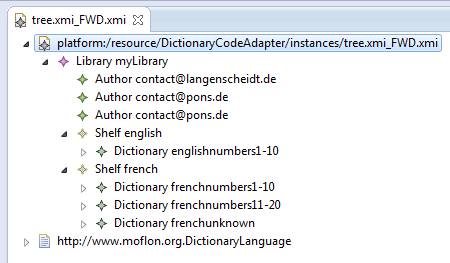
\includegraphics[width=0.7\textwidth]{eclipse_generatedForwardTransformation}
  \caption{\texttt{Dictionary} result of the forward transformation}
  \label{eclipse:generatedFwdTrsfm}
\end{center}
\end{figure}

\vspace{0.5cm}

\item[$\blacktriangleright$] Your output may or may not resemble ours. In fact, there's a 50/50 chance the any of the \texttt{author} nodes were ever created!
Let's run the eMoflon integrator on \texttt{corr\_FWD.xmi} to find out why.\footnote{If you haven't already, read Part IV, Section 6 for details on how this feature
can help you visualise and debug a transformation}

\vspace{0.5cm}

\item[$\blacktriangleright$] Proceed through the transformation until you reach the first match to an author node (Fig.~\ref{eclipse:fwdIntegrator}). Keep an
eye on the small window below -- it states that there are two possible rules that apply to the match!

\begin{figure}[htbp]
\begin{center}
  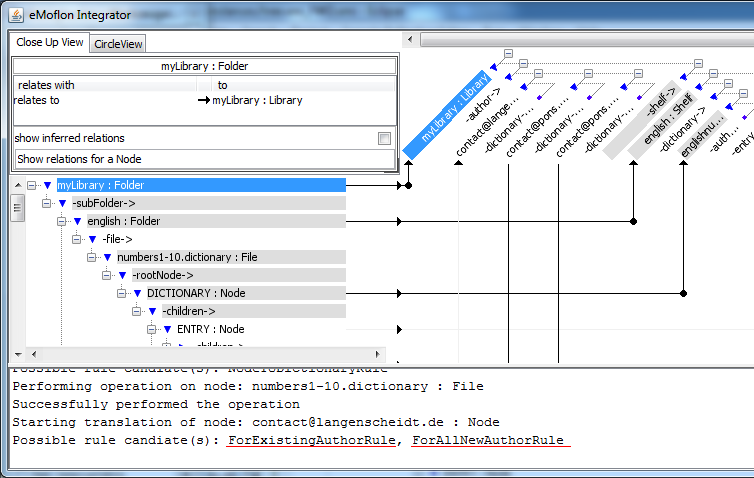
\includegraphics[width=0.8\textwidth]{eclipse_integratorAuthorChoice}
  \caption{The transformation is able to find two possible rules}
  \label{eclipse:fwdIntegrator}
\end{center}
\end{figure}

\clearpage

\item[$\blacktriangleright$] At run-time, the transformation is presented with a choice between two rules to apply to the matched \texttt{authorNode}. The
resulting choice is entirely random, meaning that your output is likely to be different each time you run \texttt{TGGMain}. For a stable transformation, you
therefore need to force a preferred decision. There are two ways to do this: (1) at run-time, where users will be able to decide for themselves what they would
prefer to use, or (2) at design-time, where you make the decision a part of the rule.

\end{itemize}

\subsubsection{Option1: Run-time decision}

The advantage with this option is that you leave users with the choice of what they would like to do. Some users don't mind having multiple authors,
while others prefer a minimalist design. They can easily change their preference here, in a configuration file.

\begin{itemize}

\item[$\blacktriangleright$] Navigate to ``DictionaryCodeAdapter/org.moflon.tie.'' Right-click this package and create
\texttt{Author\-Config\-ur\-at\-or.java}. Complete the file as described in Fig.~\ref{eclipse:authorConfig}. Be careful not to make any mistakes -- Eclipse's
auto-completion can help you here.

\begin{figure}[htbp]
\begin{center}
  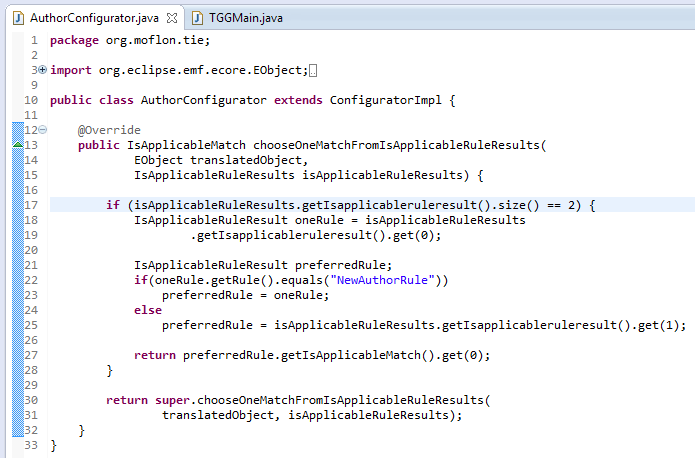
\includegraphics[width=\textwidth]{eclipse_authorConfigurator}
  \caption{Setting a preference for \texttt{NewAuthorRule}}
  \label{eclipse:authorConfig}
\end{center}
\end{figure}

\clearpage

\item[$\blacktriangleright$] As you can see on line 22, this configuration prefers to create a new author if there are two applicable results. Users can edit
this value to ``ExistingAuthorRule'' if they don't want repeated entries.

\item[$\blacktriangleright$] You still need to include the configuration as part of \texttt{TGGMain}'s execution. This decision will only arise in the forward
direction, so declare it once in \texttt{performForward} as depicted in Fig.~\ref{eclipse:editTGGMain}.

\vspace{0.5cm}

\begin{figure}[htbp]
\begin{center}
  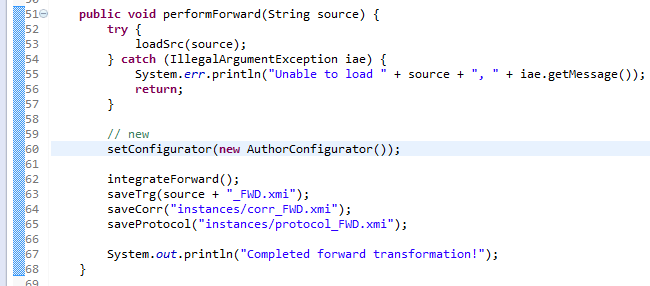
\includegraphics[width=\textwidth]{eclipse_editTGGMain}
  \caption{Invoke the configuration file to force a run-time decision}
  \label{eclipse:editTGGMain}
\end{center}
\end{figure}

\end{itemize}

\subsubsection{Option 2: Design-time decision}

This preference is built into the actual design of the transformation -- users will not be able to modify this. This decision is is implemented as a NAC,
checking to see if there is a contextual author element with the same email already present and connected to a \texttt{library}. You don't want to create this
NAC without the attribute constraint on \texttt{email} or else the transformation will create only \emph{one} author per library, which is obviously not the
desired result for the \texttt{french} shelf.

\begin{itemize}

\item[$\blacktriangleright$] Open and update either \texttt{NewAuthorRule} (Visual) as shown in Fig.~\ref{ea:existingAuthorNAC} or edit the target in 
\texttt{ForAllNewAuthorRule.tgg} (Textual) as depicted in Fig.~\ref{eclipse:existingAuthorNAC}.


\begin{figure}[htbp]
\begin{center}
  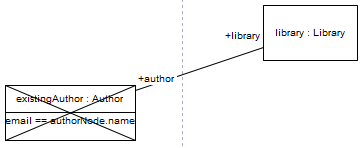
\includegraphics[width=0.7\textwidth]{ea_existingAuthorNAC}
  \caption{Add a NAC to \texttt{NewAuthorRule}}
  \label{ea:existingAuthorNAC}
\end{center}
\end{figure}

\begin{figure}[htbp]
\begin{center}
  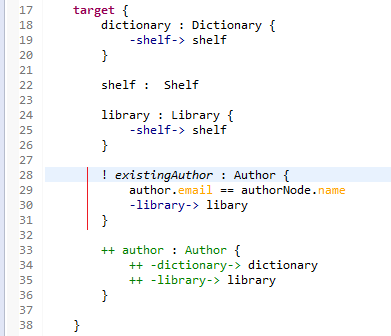
\includegraphics[width=0.7\textwidth]{eclipse_ForAllNewAuthorNAC}
  \caption{Add a NAC to \texttt{ForAllNewAuthorRule}}
  \label{eclipse:existingAuthorNAC}
\end{center}
\end{figure}

\item[$\blacktriangleright$] Save and rebuild the TGG. Run the transformation a few times, using the integrator to confirm that your preference is executed each
time. 

\end{itemize}
